% ACM sigconf short paper (arXiv preprint first; SIGIR/ECIR short or IR workshop later).
% Build: C:\Users\parvb\tools\tectonic\tectonic.exe main.tex   (or upload paper/ to Overleaf)
% Numbers in tables/ and figures/ are generated: scripts/eval_all.py -> significance.py -> make_tables.py / make_figures.py
\documentclass[sigconf,nonacm]{acmart}
\usepackage{booktabs}
\emergencystretch=1.5em
\settopmatter{printacmref=false}
\setcopyright{none}
\renewcommand\footnotetextcopyrightpermission[1]{}
\pagestyle{plain}


\begin{document}
\title{Typed Decision Models as Passage Rerankers: Effectiveness, Calibration, and Context Selection}

\author{Parv Bhargava}
\affiliation{\institution{Independent Researcher}\country{}}
\email{parvbhargavapro@gmail.com}

\begin{abstract}
Typed decision models return probabilities over caller-defined options without generating free text.
We evaluate four model families as pointwise passage rerankers on the BM25 top-100 candidates of TREC DL 2019--2023 and eight BEIR collections, examining ranking effectiveness, relevance calibration, and retrieval-augmented generation (RAG) context selection.
Jev's best format averages 56.1 nDCG@10, close to Qwen3-Reranker-8B at 56.0 and above bge-reranker-v2-m3 at 53.7, with substantial variation across collections; formal pooled equivalence depends on the inference method.
Same-base comparisons show that Clef's base model is already competitive on three tested collections, while Jeff outperforms its base under the evaluated configurations; different context budgets and prompts limit attribution to decision-model training.
On judged pairs from nine collections, Jev's raw yes/no probabilities have approximately five points lower mean ECE than bge, without target-label fitting.
Transfer-calibrated bge achieves similar mean ECE when source collections are grouped by relevance threshold.
In a RAG study on MuSiQue and NQ with three generators, Jev improves multi-hop answer quality over bge under question-ID splits with substantial MuSiQue component reuse. On 329 questions excluding directly shared components, Jev's advantage persists for top-1 and Adaptive-$k$ selection with every generator (14 of 27 comparisons pass the original Holm correction), while the smaller top-3 gains do not.
Probability thresholds, including raw thresholds with a calibration-selected readout, do not improve over fixed top-$k$ selection.
These findings establish typed decision models as competitive reranking configurations while showing that calibration alone does not guarantee better context selection.

\end{abstract}

\keywords{reranking, decision models, calibration, retrieval-augmented generation, BEIR}

\maketitle

\section{Introduction}

Retrieval-augmented generation (RAG) pipelines typically retrieve candidates with a cheap first stage, rerank them with a cross-encoder~\cite{nogueira2019monobert} or an LLM~\cite{sun2023rankgpt}, and pass a fixed top-$k$ to the generator.
Two weaknesses of this recipe are well known: cross-encoders trained on MS~MARCO transfer imperfectly to new domains~\cite{thakur2021beir}, and their scores are not probabilities~\cite{penha2021calibration}, so the cut-off $k$ is chosen by habit rather than by evidence.

A recently released class of models targets both: \emph{typed decision models} such as Jev~\cite{jev}, Cloudflare Clef~\cite{clef}, Jeff~\cite{jeff}, and Laya~\cite{laya}.
Instead of generating text, they answer a typed question about a state---a choice among named options, a yes/no (Noul) question, or an ordered scale---and return per-option probabilities. Execution differs by backend: Jeff evaluates questions in separate forward passes. Relevance judging is a natural typed task, but an explicit probability interface does not by itself establish calibration or a useful context-selection threshold.
A relevance judgment is a natural typed question (\emph{Is this passage relevant to the query?}), and a per-option probability is what a context-selection rule such as ``keep passages with $P(\text{relevant})>t$'' needs.

Evidence so far is thin: decision models have been evaluated for recommendation reranking~\cite{lyu2026jevrec} and agent-memory selection~\cite{sharma2026selection}, practitioners report Jev results on two BEIR datasets~\cite{denser2026jevqwen}, and an early audit finds that typed readouts have not yet shown an accuracy advantage over comparable label-probability readouts~\cite{tang2026tdmaudit}.
No systematic study has evaluated decision models as passage rerankers on standard IR benchmarks against cross-encoders and label-probability LLM rerankers, or measured whether their relevance probabilities are calibrated.

We provide that study, organized around three research questions.
\textbf{RQ1:} Can typed decision models, used without task-specific tuning as pointwise rerankers, match cross-encoders and label-probability LLM rerankers? 
\textbf{RQ2:} Are their relevance probabilities calibrated, with and without labels from the target collection?
\textbf{RQ3:} Do these probabilities help decide which passages a retrieval-augmented generator should see?
Our contributions are:
(1)~an evaluation of four decision-model families and three question formats, without task-specific tuning on our side, on 13 collections against cross-encoders and label-probability LLM rerankers, including same-base configuration comparisons for Clef and Jeff, paired tests, sensitivity to incomplete pools and pooled inference, and equal-context Jev--bge ablations;
(2)~a calibration analysis on nine collections with judged negatives, comparing raw readouts with source-label transfer and explicitly distinguishing numeric-threshold grouping from identical relevance semantics;
(3)~a question-ID-split RAG evaluation on MuSiQue and NQ with three generators, comparing fixed top-$k$, gap-based, and threshold-based context selection, with an analysis of \emph{which} passages each ranker selects and retrospective sensitivity to MuSiQue component reuse;
and (4)~code for reproducing and extending the evaluation, with input hashes, split IDs, complete-grid checks, and statistical sensitivity outputs.

\section{Related Work}

\paragraph{Neural and LLM reranking.}
Cross-encoders score each query--passage pair jointly~\cite{nogueira2019monobert,nogueira2020monot5} and remain the default second stage; BEIR showed that their in-domain gains shrink out of domain~\cite{thakur2021beir}.
LLM rerankers can be pointwise, pairwise, setwise, or listwise: RankGPT's sliding-window listwise prompting is competitive with supervised rerankers~\cite{sun2023rankgpt}, distilled listwise models such as RankZephyr and FIRST make this cheaper~\cite{pradeep2023rankzephyr,reddy2024first}, and setwise prompting trades off the two~\cite{zhuang2023setwise}.
Pointwise LLM rankers read relevance from the probability of a ``yes'' token and improve with graded rather than binary labels~\cite{zhuang2023beyond}; Qwen3-Reranker is a recent model trained for exactly this readout~\cite{qwen3embedding}.
Typed decision models are also pointwise, but their answer space is a declared set of options, each of which receives a probability by construction; we compare them directly with label-probability rerankers.

\paragraph{LLMs as relevance assessors.}
LLMs can predict human relevance preferences~\cite{thomas2023llmpref} and are used to generate relevance labels at scale~\cite{upadhyay2024umbrela}, with ongoing debate about the risks of doing so~\cite{faggioli2023perspectives,clarke2024cantreplace}; the LLMJudge challenge benchmarks such assessors on TREC DL~\cite{rahmani2024llmjudge}. These studies measure label agreement; we measure whether the probabilities are calibrated.

\paragraph{Typed decision models.}
Jev~\cite{jev}, its open counterparts Jeff~\cite{jeff} and Laya~\cite{laya}, and Cloudflare's Clef~\cite{clef} share a request format of a state plus typed questions.
JevBench~\cite{jevbench} ranks such models on accuracy, calibration, speed, and cost, but reports no retrieval tasks.
The closest academic work evaluates Jev for product recommendation reranking~\cite{lyu2026jevrec}; others use it to select agent-memory records~\cite{sharma2026selection}.
A study of the fine-tuned Laya typed-decisions checkpoint finds it uniformly under-confident on workflow decisions~\cite{laya2026assessor}, and Jev is reported calibrated on familiar closed-choice tasks but over-confident beyond its knowledge boundary~\cite{jev2026selfknowledge}; an early audit of 28 papers on Jev finds its clearest gains in latency and cost rather than accuracy over comparable label-probability readouts~\cite{tang2026tdmaudit}, which is the comparison our label-probability baselines make for retrieval.
Outside the literature, practitioners have reported Jev reranking results on SciFact and NFCorpus~\cite{denser2026jevqwen} and, in a pre-registered experiment on the roughly 1{,}000 MS~MARCO candidates per DL19 query, found Jev's ten-level score readout below its Noul answer and both below monoBERT (65.2, 68.4, and 71.8 nDCG@10)~\cite{carlaiau2026protocol}. We rerank only the BM25 top-100, where Jev's DL19 scores are 71.3--72.8.

\paragraph{Calibrated relevance and context selection.}
Neural rankers are known to be poorly calibrated~\cite{penha2021calibration}, as are modern neural networks generally~\cite{guo2017calibration}, and ranking losses leave the scale of scores unconstrained, which motivates scale-calibrated training~\cite{yan2022scale}; Platt scaling~\cite{platt1999} is the standard fix but needs labels. LLM rerankers' verbalized confidence in their own ranking quality is severely over-confident, although self-consistency estimates are better calibrated~\cite{ni2026predict}, and fine-tuned small LLMs can be trained to give calibrated relevance for RAG~\cite{diras2024}.
For deciding how much context a generator sees, learned selectors~\cite{meng2025dps}, score-gap heuristics~\cite{adaptivek2025}, context filtering and compression~\cite{wang2023filco,xu2024recomp,chirkova2025provence}, and retrieval evaluators that trigger corrective actions~\cite{yan2024crag} replace a fixed $k$; other work decides whether and how often to retrieve at all~\cite{asai2024selfrag,jeong2024adaptiverag}, or interleaves retrieval with reasoning for multi-hop questions~\cite{trivedi2023ircot}. Irrelevant passages and their position affect RAG answers in non-obvious ways~\cite{cuconasu2024noise,liu2024lost}.
We test whether off-the-shelf decision-model probabilities make such selection a simple threshold.

\section{Decision Models as Pointwise Rerankers}

For a query $q$ and candidate passage $d$, we send the state $\{\texttt{query}: q, \texttt{passage}: d\}$ with three typed relevance questions (Table~\ref{tab:questions}).
All three can be asked in one request (Jeff\kern0pt's server evaluates each question in a separate forward pass; Laya answers all three in one shared pass), so every decision model in our study answers all three formats in a single call per pair; the three answers are therefore not independent samples.

\begin{table}[t]
\centering
\footnotesize
\setlength{\tabcolsep}{3pt}
\caption{The three typed relevance questions (instructions and option criteria verbatim from our code) and how each answer is read out for ranking. $p_x$: probability of option $x$; $\mathbb{E}[\ell]$: probability-weighted level.}
\label{tab:questions}
\begin{tabular}{p{0.9cm}p{4.7cm}p{2.1cm}}
\toprule
Format & Question and options & Primary score \\
\midrule
Choice-3 (C3) & \emph{How relevant is the passage to the search query?} relevant: ``The passage directly answers or fully addresses the query.''; partially: ``The passage is on topic and partly addresses the query, but is incomplete or indirect.''; not\_relevant: ``The passage does not address the query.'' & $\tfrac{1}{2}(2p_\text{rel}+p_\text{part})$ \\
\addlinespace[2pt]
Noul & \emph{Does the passage answer or address the search query?} true: ``The passage answers or substantively addresses the query.''; false: ``The passage is off topic or does not help answer the query.'' & $P(\text{yes})$ \\
\addlinespace[2pt]
Score-4 (S4) & \emph{How relevant is the passage to the search query?} 0: ``Irrelevant: the passage has nothing to do with the query.''; 1: ``Related: on topic but does not answer the query.''; 2: ``Highly relevant: partly answers the query.''; 3: ``Perfectly relevant: dedicated to the query and fully answers it.'' & $\mathbb{E}[\ell]/3$ \\
\bottomrule
\end{tabular}
\end{table}

For every backend, the Score-4 value returned by the model equals the probability-weighted level $\mathbb{E}[\ell]$ computed from its option probabilities (checked on 20{,}000 answers per model; maximum deviation 0.03, from Jev's two-decimal rounding).

\paragraph{Probability readout.}
Calibration needs a probability for the \emph{binarized} relevance a collection uses.
The strict readout is $p_\text{rel}$ (C3), $P(\ell\ge2)$ (S4), or $P(\text{yes})$ (Noul); the lenient readout, for collections whose lowest relevant grade means \emph{partially} relevant, is $p_\text{rel}+p_\text{part}$ (C3) or $P(\ell\ge1)$ (S4).
We assign the lenient readout to TREC-COVID, DBPedia, and News, whose label definitions describe the lowest relevant grade as partial, and the strict readout elsewhere.
\emph{Disclosure:} this assignment was introduced after we had observed a Choice-3 ECE of 43.9 on TREC-COVID under the strict readout. It is the most favorable readout policy for Jev's Choice-3 answers (mean ECE 14.8, versus 19.2 strict everywhere and 34.8 lenient everywhere); the Noul readout does not depend on it. We therefore lead with Noul in our calibration claims, report Jev's Choice-3 under both policies in Table~\ref{tab:calibration}, and give both readouts for every collection in Appendix Table~\ref{tab:readouts}. We separately evaluate source-label transfer grouped by numeric binarization threshold (Section~\ref{sec:setup}); this grouping does not imply identical relevance semantics or the same adaptation as the readout policy.

\paragraph{Ties.}
Some decision models report probabilities rounded to two decimals, producing thousands of exact ties per collection.
To avoid \texttt{trec\_eval}'s document-ID tie-breaking, exact model-score ties use BM25 rank. Choice-3 first adds $10^{-6}p_{\mathrm{rel}}$ to the listed expected-grade score, so ties in primary expected grade are distinguished by strict relevance probability before BM25. This perturbation is part of the cached scoring configuration; the table lists its primary score.

\section{Experimental Setup}\label{sec:setup}

\paragraph{Collections and candidates.}
We use the candidates and relevance judgments of the RankGPT/RankLLM evaluation~\cite{sun2023rankgpt,rankllm} (our rerankers are pointwise, not listwise): TREC DL 2019--2023 passage~\cite{craswell2020dl19,craswell2021dl20,craswell2022dl21,craswell2023dl22,craswell2024dl23} (43/54/53/76/82 queries) and eight BEIR collections~\cite{thakur2021beir}---TREC-COVID, NFCorpus, Touche, DBPedia, SciFact, Signal, News, and Robust04 (308 DL and 1{,}525 BEIR queries, 1{,}833 in total; 15 NFCorpus queries have no BM25 candidates and score zero for every system).
Candidates are the Pyserini~\cite{pyserini} BM25 top-100 runs distributed with RankLLM, evaluated with the official Pyserini qrels; our BM25 nDCG@10 reproduces RankGPT's reported values on DL19/20 and seven of the eight BEIR collections (NFCorpus: 32.2 vs.\ 30.8).
Two caveats apply to the newer DL years: 31 of the 82 DL23 queries are synthetic (generated by T5 or GPT-4), and the DL22 judgments were propagated to near-duplicate passages; we follow common practice and keep both.
All systems rerank the full top-100 and are evaluated with \texttt{ir\_measures}~\cite{irmeasures}. We use depth 100 because it is the depth at which RankGPT and RankLLM report results on these runs, and because the strong rerankers still improve between depths 50 and 100 on TREC DL (Appendix Table~\ref{tab:depth}). Since pointwise scores are computed independently per passage, shallower depths can be simulated exactly from the same scores, and a pointwise reranker's cost grows linearly with depth.

\paragraph{Systems.}
Cross-encoders, both trained with MS~MARCO~\cite{bajaj2016msmarco} data: \texttt{ms-marco-MiniLM-L6-v2} (22M) and \texttt{bge-reranker-v2-m3} (568M, fp16)~\cite{bgererankerv2m3,chen2024bgem3}, both with a 512-token window.
Label-probability LLM rerankers, which read relevance from the probability of a ``yes'' token rather than from a typed answer: Qwen3-Reranker-0.6B, 4B, and 8B~\cite{qwen3embedding} with their official instruction template (4B and 8B with 4-bit NF4 weights to fit an 8\,GB GPU), and Qwen3-235B-A22B-Instruct-2507~\cite{qwen3} prompted pointwise for a Yes/No answer, with $P(\text{yes})$ renormalized over the Yes and No tokens among the top-5 next-token probabilities~\cite{zhuang2023beyond} (0.5 if neither appears, 1 or 0 if only one does; via OpenRouter, restricted to two fp8 deployments; DL19--23, TREC-COVID, NFCorpus, and Robust04 only, for cost).
As a same-base control we ask Clef's base model, Qwen3.8-27B, the pointwise Yes/No prompt (Cloudflare's deployment via OpenRouter, reasoning disabled; DL19, DL20, and TREC-COVID only, because the endpoint was limited to 20 requests per minute), and Jeff\kern0pt's base model, Qwen3.5-0.8B (locally, thinking disabled, on all 13 collections; $P(\text{yes})$ from the full next-token distribution).
For Qwen3-235B and Jeff's base model we also use a graded readout~\cite{zhuang2023beyond}: the same prompt asks for a 0--4 rating, and passages are ranked by the expected rating over the five digit tokens. All of these read the first 448 passage tokens, the cross-encoders' budget. Qwen3-Reranker-0.6B is close to bge-reranker-v2-m3 on average but significantly worse on DL22, DL23, and Touche.
Decision models, all used without task-specific tuning on our side: Laya (421M, ModernBERT-large~\cite{warner2024modernbert})~\cite{laya}; Jeff-Qwen3.5-0.8B v1.2~\cite{jeff}; Jev~1.13 (snapshot \texttt{20260917}) via the OpenRouter Decisions API~\cite{jev}; and Clef~27B~\cite{clef}, an open-weight decision model adapted from Qwen3.8-27B, through Cloudflare's deployment on the same API (DL19--23, TREC-COVID, and Robust04 only, for cost).
Jev is a closed model whose training data we cannot inspect; MS~MARCO, BEIR, and Robust04 are old, public collections that may overlap with it.
For reference we also quote published results on the identical BM25 top-100 runs: monoT5-3B~\cite{nogueira2020monot5} and RankGPT~\cite{sun2023rankgpt}.

\paragraph{Context budgets.}
Models read different amounts of each passage: the cross-encoders 512 tokens including the query, Laya about 320 passage tokens, Jev, Clef, and Jeff the first 4{,}000 characters ($\approx$1{,}000 tokens), and the label-probability LLMs 448 passage tokens.
On TREC DL, DBPedia, and Signal almost no passage is truncated; on the BEIR abstract collections (TREC-COVID, NFCorpus, SciFact) 29--38\% exceed the cross-encoders' budget; and on Touche, News, and Robust04 69--97\% do (Table~\ref{tab:longdoc}).
As newer-content benchmark checks we add NovelEval-2306~\cite{sun2023rankgpt} (21 queries, 20 passages each, graded 0--2) and FutureQueryEval~\cite{abdallah2025futurequery} (148 queries about events after April 2025, graded 0--2, BM25 top-100 built with \texttt{bm25s} over its 2{,}787-document corpus); they are reported separately and not included in the 13-collection averages.
For the three long-document collections we add an equal-budget condition in which every passage is cut to its first 448 tokens before any model sees it, and bge-reranker-v2-m3 at a 2{,}048-token window.

\paragraph{Metrics and tests.}
Ranking: nDCG@10 with paired two-sided $t$-tests over queries; Holm correction covers the collections available for each system--baseline pair, not the roughly 40 pairs or formats. Table averages weight collections equally. We additionally pool collection effects with DerSimonian--Laird random effects and report both normal inference and a post-hoc modified Knapp--Hartung sensitivity analysis~\cite{rover2015mkh}. mKH uses Student-$t$ with $k-1$ degrees of freedom and floors the residual variance multiplier at one. Pooled TOST with a $\pm2$ nDCG margin is exploratory: the margin was chosen after seeing results, and normal/mKH conclusions are distinguished. We also report Judged@10 and condensed nDCG$'$@10 to assess sensitivity to incomplete pools.
Calibration: ECE (15 equal-width bins) and Brier score on judged pairs from nine collections with negatives (DL19--23, TREC-COVID, DBPedia, News, Robust04), with paired query-cluster bootstrap 95\% CIs (2,000 replicates; Holm over nine collections). Transfer Platt scaling uses no target labels: All pools the other collections with equal weight per pair; Group restricts sources to the same numeric binarization threshold and weights source collections equally (DL$\to$DL, dense BEIR$\to$BEIR). Numeric thresholds need not encode identical relevance semantics, especially for partial versus strict relevance in BEIR. In-collection Platt scaling uses target labels with 10$\times$ repeated five-fold query cross-fitting and serves as a reference floor.
Because judged pairs are not a random sample of candidates, we also report ECE when unjudged candidates are treated as non-relevant (Appendix).

\paragraph{RQ3: context selection.}
We use MuSiQue-Ans dev~\cite{trivedi2022musique} (multi-hop; 20 candidate paragraphs per question, 2--4 labelled as supporting) and NQ-open test~\cite{kwiatkowski2019nq} with the DPR top-20 passages~\cite{karpukhin2020dpr} (single-hop; 18.6\% of final-set questions have no answer-bearing passage; gold labels come from DPR's string-match \texttt{has\_answer} flag).
With seed 13, each dataset is split into calibration (200), pilot (300), and final (1,000) questions with disjoint IDs. MuSiQue families were not kept together: 494 of 1,000 final questions reuse their final decomposition sub-question ID from pilot, 349 from calibration, and 578 from either (265 from both). Counting any decomposition sub-question ID, 671 final questions overlap either design split. We therefore additionally report a retrospective sensitivity analysis on the remaining 329 questions with no directly shared sub-question IDs; this is not a new confirmatory split.
The calibration set is used to fit Platt scaling on gold labels and to choose Jev's probability readout by Brier score (Noul on MuSiQue, Choice-3 strict on NQ); thresholds are therefore applied to \emph{Platt-scaled} probabilities that use target-dataset labels.
Jev ranks candidates by its Score-4 expected level, bge-reranker-v2-m3 by its logit. Policies select passages by fixed top-$k$, Adaptive-$k$ (cut at the largest gap in the ranker's own score~\cite{adaptivek2025}), a threshold $P>t$, or top-2 plus any further passage with $P>t$ (``top-2+threshold''). The nine policies compared between rankers are top-1/2/3/5, Adaptive-$k$, top-2+threshold at 0.3 and 0.5, and threshold at 0.2 and 0.3.
Three generators answer with the selected passages (temperature 0, at most 32 tokens, no option to abstain; prompt in the Appendix): Qwen2.5-7B-Instruct~\cite{qwen25}, Llama-3.1-8B-Instruct~\cite{llama3}, and Qwen3-30B-A3B-Instruct-2507, via OpenRouter. We score answers with SQuAD-normalized F1.
Policies and thresholds were fixed after the pilot before final generation. The locked threshold-rule comparisons were against top-3 and Adaptive-$k$; comparisons against top-2 and top-5 were added later and are exploratory. The pilot motivated the top-2+threshold floor. Raw thresholds (MuSiQue pilot Qwen2.5-7B: 41.6 F1 at 0.3 versus 43.9 Platt-scaled) were dropped from the lock and added after final results as a post-hoc analysis. Their probability readout still uses labelled calibration questions, so they avoid Platt fitting but are not label-free.
Comparisons are paired over questions. For each dataset and generator, Holm correction is applied separately to the nine ranker-effect tests (Jev vs.\ bge-reranker-v2-m3 under each policy) and to the four threshold-rule tests (top-2+threshold at 0.3 vs.\ top-2, top-3, top-5, and Adaptive-$k$); an earlier version of our analysis mixed the two families, and we separated them after an internal review. We add 95\% CIs and, after seeing the final results, TOST equivalence tests with a $\pm2$ F1 margin, which we report as post-hoc and without multiplicity correction.
These original question-level tests do not account for MuSiQue family dependence. For the 329-question sensitivity analysis, we keep fits, readouts, policies, and generated answers fixed and add unadjusted paired family-bootstrap 95\% percentile CIs (20,000 replicates, seed 13). Families are connected components across all 2,417 MuSiQue source questions linked by any shared decomposition ID; 212 families contain subset questions. Each replicate samples families with replacement and divides the summed paired F1 differences by the sampled question count, preserving the question-weighted estimand.

\paragraph{Hardware.}
Local models ran on a laptop RTX~4060 (8\,GB); Jeff ran through its reference server, whose attention kernels fall back to a slow reference implementation on Windows, so its latency is pessimistic.
API models were called through OpenRouter; Jev received all three questions per call. All API calls in this study cost about \$31 in total, so every experiment can be reproduced on a small budget.
OpenRouter routed the Llama and Qwen3-30B generators across several hosting providers (Qwen2.5-7B was served by one), which may serve differently quantized weights; provider assignment was balanced across policies, and we record the provider of every call.

\section{Results}

\begin{table*}[t]
\centering
\footnotesize
\setlength{\tabcolsep}{2.6pt}
\caption{nDCG@10 for reranking the BM25 top-100 (Pyserini runs and qrels, as in RankGPT/RankLLM). $^\uparrow$/$^\downarrow$: significantly better/worse than bge-reranker-v2-m3 (paired $t$-test over queries, Holm-corrected over the collections each pair was evaluated on, $p<0.05$). Best displayed configuration per column in bold; all formats and controls appear in Appendix Table~\ref{tab:ranking-full}. Averages are reported only for systems run on every collection of the group (dash otherwise); matched comparisons for Clef and the P(yes) LLMs are given in the text. Touche, News and Robust04 contain long documents that every model truncates (Table~\ref{tab:longdoc}).}
\label{tab:ranking}
\begin{tabular}{lrrrrr|r|rrrrrrrr|r|r}
\toprule
 & \multicolumn{6}{c|}{TREC Deep Learning} & \multicolumn{9}{c|}{BEIR} & \\
System & DL19 & DL20 & DL21 & DL22 & DL23 & \textit{Avg} & Covid & NFC & Touche & DBP & SciF & Signal & News & Rob04 & \textit{Avg} & \textbf{All} \\
\midrule
BM25 (first stage) & 50.6 & 48.0 & 44.6 & 26.9 & 26.2 & 39.3 & 59.5 & 32.2 & \textbf{44.2} & 31.8 & 67.9 & 33.1 & 39.5 & 40.7 & 43.6 & 41.9 \\
\addlinespace[1pt]
\multicolumn{17}{l}{\textit{Cross-encoders}} \\
MiniLM-L6 (22M) & 72.7 & 67.5 & 65.6 & 49.9 & 42.2 & 59.6 & 74.5 & 34.9 & 28.4$^\downarrow$ & 43.9 & 69.5$^\downarrow$ & \textbf{33.9}$^\uparrow$ & 44.3 & 47.3$^\downarrow$ & 47.1 & 51.9 \\
bge-reranker-v2-m3 (568M) & 72.4 & 68.1 & 66.2 & \textbf{51.4} & 45.1 & 60.6 & 78.3 & 34.3 & 38.3 & 44.0 & 75.0 & 29.0 & 43.6 & 51.9 & 49.3 & 53.7 \\
\addlinespace[1pt]
\multicolumn{17}{l}{\textit{Label-probability LLM rerankers}} \\
Qwen3-Reranker-0.6B & 69.4 & 64.0 & 65.1 & 46.3$^\downarrow$ & 38.8$^\downarrow$ & 56.7 & \textbf{86.2}$^\uparrow$ & 36.8$^\uparrow$ & 29.2$^\downarrow$ & 43.3 & 76.8 & 30.6 & 45.5 & 55.8$^\uparrow$ & 50.5 & 52.9 \\
Qwen3-Reranker-4B (4-bit) & \textbf{74.0} & 68.2 & 66.2 & 50.4 & 45.0 & 60.7 & 84.1$^\uparrow$ & 37.1$^\uparrow$ & 34.9 & \textbf{46.4}$^\uparrow$ & 77.8 & 33.8$^\uparrow$ & 48.6$^\uparrow$ & 57.4$^\uparrow$ & 52.5 & 55.7 \\
Qwen3-Reranker-8B (4-bit) & 73.6 & 66.5 & 66.2 & 51.1 & 44.9 & 60.5 & 83.8$^\uparrow$ & 37.5$^\uparrow$ & 36.2 & 45.5 & 79.2$^\uparrow$ & 33.7$^\uparrow$ & \textbf{51.6}$^\uparrow$ & 58.0$^\uparrow$ & \textbf{53.2} & 56.0 \\
Qwen3-235B, P(yes) & 68.6 & 66.5 & 65.6 & 46.2 & 42.8 & 57.9 & 80.0 & 34.6 & -- & -- & -- & -- & -- & 60.2$^\uparrow$ & -- & -- \\
Qwen3.8-27B (Clef's base), P(yes) & 73.0 & 69.8 & -- & -- & -- & -- & 83.7$^\uparrow$ & -- & -- & -- & -- & -- & -- & -- & -- & -- \\
Qwen3.5-0.8B (Jeff's base), P(yes) & 42.9$^\downarrow$ & 38.9$^\downarrow$ & 50.6$^\downarrow$ & 26.3$^\downarrow$ & 28.6$^\downarrow$ & 37.4 & 60.2$^\downarrow$ & 17.3$^\downarrow$ & 19.1$^\downarrow$ & 21.4$^\downarrow$ & 28.0$^\downarrow$ & 24.4$^\downarrow$ & 22.7$^\downarrow$ & 33.5$^\downarrow$ & 28.3 & 31.8 \\
\addlinespace[1pt]
\multicolumn{17}{l}{\textit{Laya (421M)}} \\
\quad Noul & 57.1$^\downarrow$ & 52.1$^\downarrow$ & 55.0$^\downarrow$ & 36.2$^\downarrow$ & 32.0$^\downarrow$ & 46.5 & 74.2 & 28.9$^\downarrow$ & 22.5$^\downarrow$ & 28.7$^\downarrow$ & 44.5$^\downarrow$ & 21.8$^\downarrow$ & 35.7$^\downarrow$ & 34.5$^\downarrow$ & 36.4 & 40.3 \\
\addlinespace[1pt]
\multicolumn{17}{l}{\textit{Jeff (0.8B)}} \\
\quad Noul & 59.5$^\downarrow$ & 50.1$^\downarrow$ & 52.5$^\downarrow$ & 33.0$^\downarrow$ & 30.4$^\downarrow$ & 45.1 & 67.3$^\downarrow$ & 24.5$^\downarrow$ & 23.5$^\downarrow$ & 30.0$^\downarrow$ & 46.7$^\downarrow$ & 27.4 & 33.6$^\downarrow$ & 34.1$^\downarrow$ & 35.9 & 39.4 \\
\addlinespace[1pt]
\multicolumn{17}{l}{\textit{Clef 27B (open weights, API; 7 collections)}} \\
\quad Score-4 & 72.2 & \textbf{70.2} & 69.3 & 49.1 & \textbf{46.8} & \textbf{61.5} & 84.0 & -- & -- & -- & -- & -- & -- & \textbf{66.5}$^\uparrow$ & -- & -- \\
\addlinespace[1pt]
\multicolumn{17}{l}{\textit{Jev 1.13 (API)}} \\
\quad Noul & 71.3 & 70.0 & 69.5 & 50.1 & 45.0 & 61.2 & 84.1 & 37.7$^\uparrow$ & 35.5 & 42.7 & 79.8$^\uparrow$ & 28.3 & 47.6 & 66.0$^\uparrow$ & 52.7 & 56.0 \\
\quad Score-4 & 72.8 & 69.9 & \textbf{70.0}$^\uparrow$ & 48.5 & 44.3 & 61.1 & 85.0$^\uparrow$ & \textbf{38.4}$^\uparrow$ & 31.6 & 44.5 & \textbf{80.0}$^\uparrow$ & 29.8 & 48.6 & 65.9$^\uparrow$ & 53.0 & \textbf{56.1} \\
\bottomrule
\end{tabular}
\end{table*}

\paragraph{RQ1: Effectiveness.}
Large decision models are competitive, with substantial collection variation (Table~\ref{tab:ranking}; full formats in Appendix Table~\ref{tab:ranking-full}). Jev Score-4 averages 56.1 nDCG@10 over 13 collections and Qwen3-Reranker-8B 56.0, followed by Qwen4B (55.7), bge (53.7), Qwen0.6B (52.9), MiniLM (51.9), and BM25 (41.9). Unweighted averages describe this benchmark suite; random-effects estimates instead weight effects by uncertainty and heterogeneity. With normal inference, Jev S4 minus Qwen8B is $+0.3$ (90\% CI $[-1.3,1.9]$), meeting the post-hoc $\pm2$ equivalence criterion; modified Knapp--Hartung (mKH) widens it to $[-1.4,2.0]$ (unrounded upper limit 2.02), which does not establish equivalence. Jev S4 minus bge is $+2.6$, with normal 95\% CI $[0.1,5.1]$ and mKH CI $[-0.4,5.6]$ (Appendix Table~\ref{tab:meta-sensitivity}). Large heterogeneity ($I^2\approx0.9$) limits generalization from these means. Against Qwen8B, Jev is significantly better only on Robust04 ($+7.9$) and worse on Signal ($-3.9$, Holm). Across all evaluated configurations, Clef wins DL20, DL23, and Robust04, Jev DL21, NFCorpus, and SciFact, Qwen rerankers DL19, TREC-COVID, DBPedia, and News, bge DL22, MiniLM Signal, and BM25 Touche.
On TREC DL, Jev S4 averages 61.1 versus bge 60.6 and MiniLM 59.6, significantly exceeding bge only on DL21. The normal pooled Jev--bge difference is $+0.7$ (90\% CI $[-1.2,2.6]$): this interval alone supports exploratory non-inferiority at $-2$, but not $\pm2$ equivalence. The Appendix also reports mKH sensitivity, so we do not use non-inferiority as a headline. On BEIR, Jev averages 53.0 versus bge 49.3.
Against bge-reranker-v2-m3, Jev Score-4 is significantly better on five collections (DL21, TREC-COVID, NFCorpus, SciFact, Robust04) and significantly worse on none, although on Touche, where all neural rerankers fall below BM25, it is 6.6 points lower (unadjusted $p=0.017$); against MiniLM it is significantly worse on Signal.
Robust04 contributes much of the margin: without it Jev and bge average 55.3 and 53.8 over 12 collections (pooled $+1.7$, normal 95\% CI $[0.1,3.4]$, mKH $[-0.4,3.9]$) and 51.1 and 49.0 on the other seven BEIR collections. Every LLM-based system is unusually strong on Robust04 (Jev 65.9, Clef 66.5, Qwen235B 60.2, Qwen0.6B/4B/8B 55.8/57.4/58.0, versus bge 51.9). This is consistent with either an advantage on long news articles or overlap with these public 2004 topics; we cannot separate them.
On newer-content benchmarks, Jev scores 62.5--63.5 on FutureQueryEval versus bge 58.2 ($p\le0.001$), and 90.4--91.3 on NovelEval versus 81.8 ($p\approx0.05$). Its leads over Qwen8B (61.2 and 86.2) are not significant. Both sets predate Jev's release, and its training cutoff is unknown; these results do not exclude contamination.
Published monoT5-3B results on identical candidates are 51.4 on BEIR-8 and 71.8/68.9 on DL19/20, versus Jev S4 53.0 and 72.8/69.9~\cite{sun2023rankgpt}; without Robust04 the BEIR averages are 50.6 and 51.1. This comparison is descriptive because published per-query outputs are unavailable. RankLLM reports DL19--23 averages of 62.1 for RankZephyr-7B, 61.0 for DuoT5, and 60.4 for monoT5, versus Jev S4 61.1~\cite{rankllm}. Our 4-bit RankZephyr DL19 check scores 72.5 versus the published 74.1. Published GPT-4 BEIR results use GPT-3.5's top-30 and are not directly comparable.

Clef averages 64.4--65.4 across formats on seven collections versus Jev 64.1--65.2 and bge 61.9. Jev S4 minus Clef S4 has a normal pooled 95\% CI $[-1.0,0.4]$; exploratory $\pm2$ equivalence holds across formats under normal and mKH inference. The three formats share a call, so these are related comparisons.
Qwen235B's $P(\text{yes})$ averages 58.1 on eight collections versus Jev Noul 61.7; Jev is significantly better on five and worse on none. A graded 0--4 readout raises Qwen235B to 59.8 ($+1.8$, normal pooled 95\% CI $[0.8,2.8]$), closer to Jev S4 61.8.
Same-base comparisons assess configurations rather than isolate training. On DL19, DL20, and TREC-COVID, Clef's base Qwen3.8-27B averages 75.5 as $P(\text{yes})$ versus Clef 74.8--75.5; none of nine collection-level differences is significant. Clef S4 meets normal $\pm2$ equivalence ($p=0.005$), but the mKH 90\% CI $[-2.2,2.3]$ does not. We find no measurable ranking benefit for Clef over its base on these three collections under the tested configurations. The base itself exceeds Qwen235B by 3.3--4.4 points on each. These observations are consistent with the early audit's caution about attributing quality to typed readouts~\cite{tang2026tdmaudit}.
Jev's base, size, and training data are unknown. Its 4,000-character context also differs from the label-probability controls' 448 tokens: on Robust04 its Noul lead over Qwen235B shrinks from 5.7 to 2.4 at equal passage budget.
Jeff's formats average 39.1--39.4 over 13 collections versus its base's 31.8 (graded base: 26.4). They exceed the yes/no base significantly on 7--8 collections and are worse on none. Jeff therefore outperforms its base under the evaluated configurations; different contexts, prompts, and schemas prevent attributing the full approximately 7.5-point gain to training.

Small decision models remain below BM25 at depth 100: Laya and Jeff average 39.1--41.2 versus 41.9. Their lower Judged@10 (DL 76--81\% versus bge 96\%) and higher condensed nDCG$'$ (58.6/57.3 versus BM25 51.8 and bge 64.0) show sensitivity to incomplete pools. Laya's BEIR nDCG falls from 43.7 at depth 10 to 37.4 at depth 100, while condensed nDCG rises from 60.4 to 61.9 and Judged@10 falls from 57\% to 48\%. These diagnostics do not establish whether the unjudged passages are relevant or that pooling causes the degradation.
Jev has DL Judged@10 90.0\% and condensed all-collection nDCG 66.9 versus bge 64.0. Removing unjudged passages does not establish their relevance, so the standard score cannot be called conservative from this evidence alone.
Within a family, the three formats differ by at most 1.3 average points. Differences between backends exceed differences among these formats; this does not isolate model capacity.

\begin{table}[t]
\centering
\small
\setlength{\tabcolsep}{3pt}
\caption{Long-document collections. Top: share of candidate passages longer than each model's passage budget (XLM-R tokens; Laya English $\approx$320, cross-encoders 448 at a 512 window, bge at 2{,}048 tokens, Jev/Jeff 4{,}000 characters). Bottom: nDCG@10 with each model's own window and with every passage cut to the same first 448 tokens (``=448''). $\Delta$: Jev Score-4 minus bge at equal budget (paired $t$-test).}
\label{tab:longdoc}
\begin{tabular}{lrrr}
\toprule
 & Touche & News & Robust04 \\
\midrule
\multicolumn{4}{l}{\textit{Passages truncated (\%)}} \\
\quad Laya ($>$320 tok) & 77 & 99 & 96 \\
\quad cross-enc.\ ($>$448 tok) & 69 & 97 & 92 \\
\quad bge-2048 ($>$2{,}000 tok) & 5 & 22 & 25 \\
\quad Jev/Jeff ($>$4k chars) & 43 & 75 & 72 \\
\midrule
\multicolumn{4}{l}{\textit{nDCG@10}} \\
\quad BM25 & 44.2 & 39.5 & 40.7 \\
\quad MiniLM (512) & 28.4 & 44.3 & 47.3 \\
\quad MiniLM (=448) & 29.2 & 43.5 & 47.4 \\
\quad bge (512) & 38.3 & 43.6 & 51.9 \\
\quad bge (=448) & 38.1 & 44.6 & 51.5 \\
\quad bge (2{,}048) & 37.5 & 47.8 & 51.6 \\
\quad Jev S4 (4k chars) & 31.6 & 48.6 & 65.9 \\
\quad Jev S4 (=448) & 28.2 & 49.4 & 63.1 \\
\midrule
$\Delta$ Jev$-$bge (=448) & -9.9$^{*}$ & +4.9$^{*}$ & +11.5$^{*}$ \\
\bottomrule
\end{tabular}
\end{table}

\paragraph{Long documents.}
At the same first 448 passage tokens, Jev S4 exceeds bge by $+11.5$ on Robust04 and $+4.9$ on News ($p<0.01$, Holm over three collections), versus $+13.9$ and $+5.0$ with full context, and loses on Touche ($-9.9$; Table~\ref{tab:longdoc}). These ablations concern Jev--bge and do not establish pooled equal-context equivalence with Qwen8B.
Giving bge-reranker-v2-m3 a 2{,}048-token window, which reads most documents in full, essentially closes the gap on News (47.8) but does not help on Robust04 (51.6 vs.\ 51.9).

\begin{table}[t]
\centering
\footnotesize
\setlength{\tabcolsep}{1.6pt}
\caption{Calibration of $P(\text{relevant})$ on the nine collections with judged negatives (DL19--23, TREC-COVID, DBPedia, News, Robust04; unweighted mean over collections, ECE$\times$100, 15 bins, judged pairs only). Raw: no recalibration. Transfer (no target labels): Platt scaling fit on the other eight collections pooled (All) or only on the same numeric-threshold group, balancing source collections (Group: DL$\to$DL, BEIR$\to$BEIR); the group need not share identical relevance semantics. All weights pairs equally. In-coll.: Platt with 10$\times$ repeated 5-fold query cross-fitting on the target collection (needs target labels; SD $\le$0.6). C3/S4: Choice-3/Score-4. $^\dagger$Strict readout on every collection instead of the per-collection policy (Section~\ref{sec:setup}). $^\ast$Seven of the nine collections (no DBPedia, News). Bold: best among systems on all nine.}
\label{tab:calibration}
\begin{tabular}{lrrrrrr}
\toprule
 & \multicolumn{4}{c}{ECE} & & \\ \cmidrule(lr){2-5}
 & & \multicolumn{2}{c}{Transfer} & & & \\ \cmidrule(lr){3-4}
System & Raw & All & Group & In-coll. & Brier & $\bar{p}$ \\
\midrule
MiniLM-L6 & 35.4 & 16.8 & 8.7 & 3.0 & 0.345 & 0.58 \\
bge-v2-m3 & 20.0 & 14.9 & 6.9 & 2.6 & 0.215 & 0.39 \\
Qwen3-Rer.-0.6B & 36.1 & 17.9 & 9.6 & 2.4 & 0.357 & 0.62 \\
Qwen3-Rer.-4B & 26.9 & 19.0 & 9.2 & 2.4 & 0.265 & 0.47 \\
Qwen3-Rer.-8B & 21.6 & 17.5 & 9.6 & 2.5 & 0.221 & 0.41 \\
Qwen3-235B P(yes)$^\ast$ & 20.5 & 10.5 & 9.5 & 3.1 & 0.211 & 0.39 \\
Laya C3 & 11.0 & 7.5 & 9.3 & 2.3 & 0.184 & 0.36 \\
Laya Noul & \textbf{10.7} & 10.7 & 9.5 & 2.2 & 0.185 & 0.35 \\
Jeff C3 & 15.3 & \textbf{5.2} & \textbf{5.9} & 2.5 & 0.195 & 0.46 \\
Jeff Noul & 25.6 & 11.7 & 8.6 & \textbf{2.2} & 0.253 & 0.56 \\
Clef C3$^\ast$ & 7.8 & 8.3 & 10.4 & 3.3 & 0.134 & 0.28 \\
Clef Noul$^\ast$ & 12.5 & 12.4 & 7.3 & 2.7 & 0.146 & 0.36 \\
Clef S4$^\ast$ & 11.6 & 8.9 & 9.1 & 2.7 & 0.139 & 0.40 \\
Jev C3 & 14.8 & 9.1 & 8.9 & 4.4 & \textbf{0.169} & 0.36 \\
Jev C3 (strict)$^\dagger$ & 19.2 & 15.1 & 9.1 & 3.6 & 0.206 & 0.18 \\
Jev Noul & 15.0 & 14.2 & 6.8 & 3.0 & 0.170 & 0.38 \\
Jev S4 & 25.4 & 8.2 & 7.9 & 5.0 & 0.240 & 0.55 \\
\midrule
\multicolumn{7}{l}{\footnotesize Base rate of relevance (mean over the nine collections): 0.31} \\
\bottomrule
\end{tabular}
\end{table}

\begin{figure}[t]
\centering
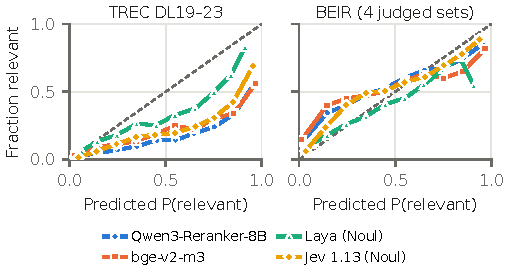
\includegraphics[width=\columnwidth]{figures/reliability.pdf}
\caption{Raw reliability on judged candidate pairs for bge, Qwen3-Reranker-8B, and the Noul readouts of Laya and Jev. Pooled within DL19--23 (left) and the four BEIR collections with negatives (right); 10 equal-width bins, hiding bins with fewer than 15 pairs. Noul needs no strict/lenient policy choice. Decision models are closer to the diagonal on DL; BEIR behavior is mixed.}
\label{fig:reliability}
\end{figure}

\paragraph{RQ2: Calibration.}
Raw cross-encoder scores were never meant to be probabilities, so we compare raw probabilities and probabilities after \emph{transfer} calibration, which uses no labels of the target collection (Table~\ref{tab:calibration}).
Jev and Laya's raw Noul probabilities improve calibration on judged candidate pools without target-label fitting. Jev Noul has mean ECE 5.0 points below bge (paired query-bootstrap 95\% CI $[-6.3,-3.9]$), lower on eight of nine collections, significantly lower on five after Holm, and significantly higher on none. TREC-COVID is slightly higher ($+0.17$). Laya Noul is 9.2 points lower ($[-10.8,-7.5]$). Jeff Noul is an exception: its ECE is 25.6 versus bge 20.0.
On DL, trained rerankers over-predict relevance (ECE 51.1/36.5/27.6 for Qwen0.6B/4B/8B, 47.0 for MiniLM, and 23.1 for bge; Figure~\ref{fig:reliability}).
For C3, the per-collection policy gives Jev a 5.1-point ECE advantage over bge ($[-7.1,-3.4]$), while strict everywhere gives $-0.7$ ($[-2.5,0.9]$). Jev's DBPedia ECE is worse by 9.9 under the policy and 14.1 under strict; Robust04 is worse by 0.9 under both.
These differences are insensitive to the number of bins (5--30) and to equal-mass binning (within 0.4 points). A Brier decomposition shows that Jev's advantage comes from both reliability (0.036 vs.\ 0.067 for Choice-3) and resolution (0.060 vs.\ 0.045).
Jev's Score-4 probabilities over-predict relevance under the per-collection policy (mean prediction 0.55 against a base rate of 0.31), because the lenient readout $P(\ell\ge1)$ counts ``related but not answering'' as relevant. Read strictly, they are better calibrated than bge-reranker-v2-m3 ($-2.1$, $[-3.4,-0.9]$).

Source-label transfer can give bge similar mean ECE. Pair-pooled transfer yields bge 14.9 and MiniLM 16.8, versus Jev C3/S4/Noul 9.1/8.2/14.2 and Laya C3 7.5. Collection-balanced pooling changes little.
Within-group transfer restricts sources by numeric binarization threshold and balances collections: DL$\to$DL and dense BEIR$\to$BEIR. This yields bge ECE 6.9, similar to Jev Noul 6.8, versus Jev C3 8.9 and Laya C3 9.3. The BEIR group mixes partial-relevance definitions with strict Robust04, so this is not identical semantic adaptation.
These descriptive means do not establish calibration equivalence; they show that source-label transfer can close the average raw-calibration gap on this suite.
On seven shared API collections, Clef C3 has raw ECE 7.8 and Brier 0.134 versus Jev C3 ECE 12.5 and bge 20.2. On three base-control collections, Clef Noul ECE is 13.1 versus its base 14.6, while C3 is 7.8. Jeff Noul ECE is 25.6 versus its base 26.5 across nine, and Jeff C3 is 15.3. These are configuration comparisons, not isolated training effects. Qwen235B's raw yes/no ECE is 20.5; transfer reduces it to 10.5 versus Jev Noul 13.0 on shared collections.
Calibration is conditional on judged candidates, whose mean base rate is 0.31. Treating unjudged candidates as negatives preserves the raw advantage of Jev Noul and Laya Noul, but reverses Jeff C3's advantage; Jeff Noul is worse already on judged pairs (Appendix Table~\ref{tab:judged}).

\paragraph{Efficiency.}
Per query--passage pair, the local cross-encoders and Qwen3-Reranker-0.6B take 0.3--14\,ms (median) on a laptop GPU, Qwen3-Reranker-4B and 8B 102 and 148\,ms (4-bit), Laya 58\,ms, and Jeff 100\,ms (with slow reference kernels); the API models take a median 176\,ms (Jev), 401\,ms (Clef), and 850\,ms (Qwen3-235B) per call with 8--24 concurrent requests. Reranking 100 passages costs \$3.4 per 1k queries with Jev on average (\$2.4--5.7; long documents cost more) and \$2.3 with the Qwen3-235B yes/no baseline; on the seven collections where both were run, Clef 27B costs about 4.8 times as much as Jev (\$15.3 vs.\ \$3.2).

\begin{table*}[t]
\centering
\footnotesize
\setlength{\tabcolsep}{4pt}
\caption{RQ3: answer F1 on the original 1{,}000 ID-disjoint final questions per dataset; MuSiQue component families overlap design splits. Avg.\ $n$: mean number of selected passages (independent of generator). $^\dagger$: Jev significantly better than bge-reranker-v2-m3 under the same policy in the original question-level paired $t$-test (Holm-corrected, $p<0.05$); these tests do not account for family dependence. Displayed policies and ranker-effect comparisons were fixed after separate pilot questions. Thresholds use a readout selected with labelled calibration questions; the $P>0.3$ rows are Platt-scaled.}
\label{tab:rag}
\begin{tabular}{lrrrrrrrr}
\toprule
 & \multicolumn{3}{c}{MuSiQue} & \multicolumn{3}{c}{NQ} & \multicolumn{2}{c}{Avg.\ $n$} \\
Policy & Qwen2.5-7B & Llama-3.1 & Qwen3-30B & Qwen2.5-7B & Llama-3.1 & Qwen3-30B & MuSiQue & NQ \\
\midrule
No context & 10.5 & 9.3 & 12.6 & 26.7 & 31.4 & 35.2 & 0.0 & 0.0 \\
All 20 passages & 38.8 & 37.0 & 46.3 & 52.5 & 49.4 & 51.5 & 20.0 & 20.0 \\
Gold passages (oracle) & 60.9 & 54.7 & 64.1 & 60.2 & 59.1 & 59.7 & 2.6 & 3.4 \\
\multicolumn{9}{l}{\textit{Jev 1.13}} \\
\quad top-1 & 45.2$^\dagger$ & 36.4$^\dagger$ & 43.4$^\dagger$ & 50.4 & 50.4$^\dagger$ & 51.4 & 1.0 & 1.0 \\
\quad top-3 & 44.6$^\dagger$ & 39.3$^\dagger$ & 47.1$^\dagger$ & 52.1 & 50.5 & 52.9 & 3.0 & 3.0 \\
\quad top-5 & 42.4$^\dagger$ & 40.7$^\dagger$ & 47.9$^\dagger$ & 51.9 & 50.9 & 53.0 & 5.0 & 5.0 \\
\quad adaptive-$k$ & 46.7$^\dagger$ & 40.2$^\dagger$ & 47.2$^\dagger$ & 52.3 & 50.1 & 52.3 & 2.9 & 6.2 \\
\quad $P>0.3$ & 43.6$^\dagger$ & 36.1$^\dagger$ & 43.5$^\dagger$ & 51.2 & 51.5 & 52.3 & 2.4 & 2.9 \\
\quad top-2 $+$ $P>0.3$ & 44.2$^\dagger$ & 39.1$^\dagger$ & 45.2$^\dagger$ & 51.8 & 51.0 & 53.2 & 3.0 & 3.5 \\
\multicolumn{9}{l}{\textit{bge-reranker-v2-m3}} \\
\quad top-1 & 22.0 & 18.0 & 23.7 & 47.9 & 47.1 & 49.1 & 1.0 & 1.0 \\
\quad top-3 & 38.5 & 31.5 & 39.1 & 51.4 & 50.5 & 52.6 & 3.0 & 3.0 \\
\quad adaptive-$k$ & 30.5 & 26.1 & 32.6 & 50.6 & 50.5 & 51.8 & 3.1 & 7.1 \\
\quad top-2 $+$ $P>0.3$ & 35.7 & 30.4 & 37.9 & 51.3 & 51.2 & 52.6 & 2.9 & 3.9 \\
\bottomrule
\end{tabular}
\end{table*}

\paragraph{RQ3: Context selection.}
Table~\ref{tab:rag} reports answer F1 on the original 1{,}000 ID-disjoint final questions per dataset; MuSiQue component families overlap design splits.
\emph{Ranking quality helps on the original multi-hop split.} On MuSiQue, passages selected by Jev beat those selected by bge-reranker-v2-m3 under every policy and with every generator, by $+2.6$ to $+23.2$ F1. All 27 comparisons pass the original question-level Holm tests (nine policies, three generators; Table~\ref{tab:rag} shows a subset), which assume independent questions despite family reuse. With Qwen2.5-7B, Jev's single top passage (45.2) or its Adaptive-$k$ selection of 2.9 passages (46.7) beats giving the generator all 20 candidates (38.8) with a small fraction of the generator input tokens. This saving excludes the cost of scoring all 20 candidates.
This coincides with a difference in \emph{which} passage each ranker puts first. bge-reranker-v2-m3's top passage is a supporting paragraph slightly more often (88.0\% vs.\ 82.2\%, McNemar $p<10^{-4}$), but usually the first hop---the one that shares the question's entities (61.9\%)---whereas Jev's top passage is the last, answer-bearing hop in 51.2\% of questions against 15.2\% ($p<10^{-80}$; Appendix Table~\ref{tab:ragsel}), and 56--64\% across Jev's three readouts.
Changing Qwen0.6B's instructions to relevant, answers, or contains the answer yields only 16.5--18.5\% last-hop@1 and 51--56\% first-hop@1. These tested wording changes do not reproduce Jev's preference, but do not establish its cause.
Replacing gold-answer strings with \texttt{[MASKED]} reduces Jev S4 last-hop@1 to 43.8\% (Noul: 50.3\%) versus unmasked 51.2\% (56.4\%); masked bge scores 13.4\%. This is a descriptive perturbation: the marker appears in 999 of 1,000 last-hop paragraphs but only 1,621 of 19,988 candidates, revealing answer location. Residual preference may use that cue, prior entity knowledge, or memorized chains; masking cannot isolate question resolution from these explanations.
On NQ, only one of the 27 ranker-effect comparisons is significant. The full downstream comparison is against bge; Qwen0.6B appears only in the selection diagnostic, and no RAG advantage over Qwen8B is established.
\begin{table}[t]
\centering\footnotesize\setlength{\tabcolsep}{3pt}
\caption{Retrospective MuSiQue sensitivity on 329 questions with no sub-question ID in calibration or pilot. Answer F1 under three ranker-effect policies; $\Delta$ is Jev minus bge. CIs resample 212 source-graph families (20,000 paired replicates, seed 13), retaining question weights; intervals are unadjusted. $^\dagger$: passes the original nine-policy question-level Holm correction (top-1 and Adaptive-$k$ for every generator; no top-3 comparison).}
\label{tab:rag-clean}
\begin{tabular}{llrrrr}
\toprule
Generator & Policy & Jev & bge & $\Delta$ & Family 95\% CI \\
\midrule
Qwen2.5-7B & top-1 & 41.8 & 23.1 & $+18.8^\dagger$ & $[14.0, 23.8]$ \\
 & Adaptive-$k$ & 42.1 & 31.3 & $+10.7^\dagger$ & $[5.9, 15.7]$ \\
 & top-3 & 43.6 & 41.3 & $+2.4$ & $[-2.6, 7.3]$ \\
\addlinespace[2pt]
Llama-3.1-8B & top-1 & 35.0 & 20.6 & $+14.4^\dagger$ & $[9.6, 19.2]$ \\
 & Adaptive-$k$ & 38.4 & 27.1 & $+11.3^\dagger$ & $[7.1, 15.7]$ \\
 & top-3 & 41.1 & 35.7 & $+5.5$ & $[1.0, 10.0]$ \\
\addlinespace[2pt]
Qwen3-30B-A3B & top-1 & 43.9 & 26.0 & $+17.9^\dagger$ & $[12.5, 23.4]$ \\
 & Adaptive-$k$ & 47.9 & 34.6 & $+13.3^\dagger$ & $[9.0, 17.8]$ \\
 & top-3 & 48.1 & 42.4 & $+5.7$ & $[0.8, 10.5]$ \\
\bottomrule
\end{tabular}
\end{table}

\emph{Retrospective component-clean sensitivity.} On the 329 questions with no sub-question ID directly shared with calibration or pilot, top-3 Jev/bge F1 is 43.6/41.3, 41.1/35.7, and 48.1/42.4 for Qwen2.5-7B, Llama-3.1-8B, and Qwen3-30B-A3B, respectively (Table~\ref{tab:rag-clean}). Gains shrink to $+2.4$, $+5.5$, and $+5.7$; none passes the original nine-policy question-level Holm correction. Family-bootstrap intervals are $[-2.6,7.3]$, $[1.0,10.0]$, and $[0.8,10.5]$, without multiplicity correction. Jev's point estimates remain higher under all nine shared policies ($+0.5$ to $+18.8$), and 14 of 27 original-style Holm tests pass, versus 27 on the full split. The passing tests include top-1 ($+14.4$ to $+18.8$) and Adaptive-$k$ ($+10.7$ to $+13.3$) for every generator, whose family-bootstrap intervals all exclude zero (Table~\ref{tab:rag-clean}); the gain shrinks most for top-3. The top-2+$P>0.3$ rule differs from Jev top-3 by $-1.5$, $+0.5$, and $-1.8$ F1; family intervals cross zero for every generator, as do comparisons with Adaptive-$k$. This sensitivity does not quantify overlap-induced inflation: subset size and case mix change. Moreover, 23 subset questions remain indirectly connected to design questions through other source records, so direct component exclusion does not establish full family isolation or absence of model-training contamination.
\emph{Thresholds on probabilities do not beat fixed $k$.} A pure threshold at 0.3 on Platt-scaled probabilities leaves the generator with no passage for 10.3\% of MuSiQue and 21.6\% of NQ questions, which then fall back to closed-book answering (the prompt does not allow abstention).
Raw $P>0.3$ on NQ is within 1.3 F1 of the Platt threshold and top-3 for every generator; on MuSiQue it selects nothing for 25\% and is 3.4--5.9 F1 below top-3. These post-hoc raw thresholds still use a readout chosen using labelled calibration questions (Appendix~\ref{app:extra}).
In a post-hoc equivalence analysis (TOST, $\pm2$ F1), the top-2+threshold rule is equivalent to top-2, top-3, top-5, and Adaptive-$k$ on NQ for every generator; on MuSiQue it is equivalent to top-2 (and, for Llama, to top-3), and pooled over generators it is 1.9 F1 below Adaptive-$k$ (95\% CI $[-3.4,-0.4]$; Holm-adjusted $p=0.065$). On MuSiQue it is also below Adaptive-$k$ for Qwen2.5-7B ($-2.6$) and below top-3 and top-5 for Qwen3-30B-A3B ($-1.9$, $-2.7$; unadjusted $p=0.01$--$0.05$, none significant after Holm), so ``equivalent or slightly worse'' is the fair summary. It selects exactly two passages for 61\% of MuSiQue and 55\% of NQ questions but more on the rest, 3.0 and 3.5 on average, so it saves no tokens over top-3.
On these data, Jev's practical advantage over bge is chiefly ranking; neither Platt-scaled nor calibration-selected raw thresholds establish improved context selection.

\section{Conclusion}

Large typed decision models are competitive pointwise passage rerankers under the evaluated configurations. Jev's average nDCG@10 is close to Qwen3-Reranker-8B and higher than bge-reranker-v2-m3, although pooled superiority and equivalence are sensitive to small-sample inference and collection heterogeneity. Its gains over bge persist at equal passage budgets on News and Robust04; this ablation does not establish equal-context equivalence with Qwen8B. Clef performs similarly to Jev on seven collections and to its own base on three; Jeff outperforms its base, but context and prompt differences prevent attributing the entire gain to decision-model training.
Jev and Laya's raw yes/no probabilities are better calibrated than bge scores on the nine judged candidate pools. A cross-encoder calibrated on other collections in the same numeric-threshold group reaches similar mean ECE. Small open decision models remain weak deep rerankers under standard evaluation.
For RAG, Jev improves multi-hop answer quality over bge with all three generators on the original question-ID split and more often ranks the final supporting passage first. Substantial MuSiQue component reuse limits that evidence: on the retrospective 329-question component-clean subset, the top-1 and Adaptive-$k$ gains remain large ($+10.7$ to $+18.8$ F1, family-bootstrap intervals above zero for every generator), while the smaller top-3 gains do not pass the original Holm correction. Probability thresholds do not establish a gain over fixed top-$k$ on either analysis; even the raw-threshold readout was selected using labelled calibration questions.

\paragraph{Limitations.}
We use BM25 candidates, one prompt per format, and no task-specific fine-tuning on our side. Qwen3-Reranker-4B/8B use 4-bit weights, and most listwise comparisons use published results. Same-base configurations differ in context budgets and prompts; the three formats share a call. Pooled equivalence margins were chosen after observing results, and normal and small-sample inference differ on borderline comparisons. Calibration is conditional on judged candidates; numeric-threshold transfer groups need not share identical relevance semantics. The per-collection readout was chosen after observing one collection, and both readouts are reported. Jev's training data and cutoff are unknown; Robust04, MuSiQue, NovelEval, and FutureQueryEval all predate its release, so contamination remains possible. Gold-answer masking supplies an answer-location marker and cannot isolate reasoning from memorization. We retain DL23 synthetic queries and DL22 propagated judgments. Clef and the 235B baseline cover subsets; the full RAG comparison covers bge, with Qwen0.6B used only in a selection diagnostic, and does not establish an advantage over Qwen8B. RAG split IDs are disjoint, but MuSiQue component families overlap calibration and pilot extensively; the retrospective subset changes case mix and still has indirect family connections. Original question-level tests do not account for this dependence. Thresholds use target calibration labels, and the generator cannot abstain. Hardware and serving differ, so latency is indicative; generator input savings exclude the cost of scoring all candidates.

\bibliographystyle{ACM-Reference-Format}
\bibliography{refs}

\appendix
\section{Additional Results}

Table~\ref{tab:depth} reports effectiveness as a function of reranking depth; Table~\ref{tab:readouts} reports both probability readouts for every collection with judged negatives; Table~\ref{tab:judged} reports pool coverage and the pool-bias check for calibration; Table~\ref{tab:ragsel} reports generator-free selection quality for RQ3.
Code, prompts, and aggregate results are available in the reproduction repository (Declarations). All inputs are public and are downloaded by the code; the RAG splits are regenerated from a fixed seed, and the scripts reproduce every table and figure from the model outputs.

\begin{table*}[tp]
\centering
\scriptsize
\setlength{\tabcolsep}{3pt}
\caption{nDCG@10 when only the BM25 top-$k$ is reranked (simulated exactly from the pointwise scores; passages below rank $k$ keep their BM25 order). Averages over TREC DL19--23 and BEIR-8. The cost of a pointwise reranker grows linearly with $k$. BM25 alone: DL 39.3, BEIR 43.6.}
\label{tab:depth}
\begin{tabular}{lrrrrr|rrrrr}
\toprule
 & \multicolumn{5}{c|}{DL19--23} & \multicolumn{5}{c}{BEIR-8} \\
System & $k$=10 & $k$=20 & $k$=30 & $k$=50 & $k$=100 & 10 & 20 & 30 & 50 & 100 \\
\midrule
MiniLM & 43.3 & 50.8 & 53.8 & 56.7 & 59.6 & 44.9 & 46.5 & 46.6 & 46.8 & 47.1 \\
bge-v2-m3 & 43.7 & 51.6 & 54.6 & 57.8 & 60.6 & 45.9 & 48.4 & 48.7 & 49.3 & 49.3 \\
Qwen3-Rer.-0.6B & 42.9 & 49.5 & 52.0 & 54.1 & 56.7 & 45.7 & 48.4 & 49.2 & 50.0 & 50.5 \\
Laya C3 & 41.8 & 46.2 & 46.9 & 48.0 & 47.3 & 43.7 & 43.1 & 41.5 & 39.6 & 37.4 \\
Jeff Noul & 41.9 & 46.1 & 46.3 & 46.7 & 45.1 & 43.1 & 42.3 & 40.5 & 38.8 & 35.9 \\
Jev S4 & 44.0 & 51.9 & 55.1 & 58.0 & 61.1 & 46.8 & 50.4 & 51.4 & 52.5 & 53.0 \\
\midrule
\multicolumn{11}{l}{\textit{BEIR-8: condensed nDCG$'$@10 (left), Judged@10 in \% (right)}} \\
MiniLM & 60.8 & 62.3 & 62.9 & 63.6 & 64.2 & 57 & 58 & 57 & 56 & 56 \\
bge-v2-m3 & 61.2 & 63.4 & 64.1 & 65.1 & 65.7 & 57 & 57 & 57 & 56 & 55 \\
Qwen3-Rer.-0.6B & 61.4 & 63.8 & 64.9 & 66.0 & 66.9 & 57 & 57 & 57 & 57 & 56 \\
Laya C3 & 60.4 & 61.5 & 61.7 & 61.9 & 61.9 & 57 & 55 & 53 & 51 & 48 \\
Jeff Noul & 60.2 & 61.1 & 61.0 & 61.3 & 60.8 & 57 & 55 & 53 & 51 & 48 \\
Jev S4 & 61.6 & 64.8 & 66.2 & 67.7 & 69.1 & 57 & 58 & 57 & 56 & 56 \\
\bottomrule
\end{tabular}
\end{table*}
\begin{table*}[tp]
\centering
\scriptsize
\setlength{\tabcolsep}{2.2pt}
\caption{ECE$\times$100 of Choice-3/Score-4 probabilities under the strict (s) and lenient (l) readouts. The readout used in the main text is underlined. Noul has a single readout.}
\label{tab:readouts}
\begin{tabular}{llrrrrrrrrr}
\toprule
System & & DL19 & DL20 & DL21 & DL22 & DL23 & Covid & DBP & News & Rob04 \\
\midrule
Laya C3 & s & \underline{14.1} & \underline{6.4} & \underline{7.3} & \underline{8.3} & \underline{12.1} & 25.4 & 16.1 & 14.3 & \underline{5.6} \\
 & l & 24.5 & 34.0 & 36.6 & 42.9 & 41.9 & \underline{6.9} & \underline{16.7} & \underline{22.0} & 30.4 \\
Jeff C3 & s & \underline{7.1} & \underline{15.9} & \underline{12.3} & \underline{17.6} & \underline{17.3} & 25.9 & 3.3 & 14.9 & \underline{11.0} \\
 & l & 36.3 & 45.3 & 42.8 & 48.6 & 47.7 & \underline{11.6} & \underline{21.0} & \underline{23.9} & 48.2 \\
Jev C3 & s & \underline{12.9} & \underline{9.3} & \underline{13.1} & \underline{8.2} & \underline{14.3} & 43.9 & 26.7 & 30.6 & \underline{14.2} \\
 & l & 37.7 & 47.4 & 47.6 & 48.2 & 52.4 & \underline{15.8} & \underline{22.6} & \underline{23.2} & 18.6 \\
Jev S4 & s & \underline{15.8} & \underline{23.5} & \underline{24.8} & \underline{20.1} & \underline{26.7} & 13.8 & 9.7 & 19.5 & \underline{7.2} \\
 & l & 52.8 & 68.0 & 59.8 & 70.3 & 69.3 & \underline{27.4} & \underline{42.6} & \underline{40.6} & 32.3 \\
\bottomrule
\end{tabular}
\end{table*}
\begin{table*}[tp]
\centering
\scriptsize
\setlength{\tabcolsep}{2.5pt}
\caption{Pool coverage and pool-bias checks. Judged@10 (\%) and condensed (judged-only) nDCG$'$@10, averaged over the collections each system was run on; ECE$\times$100 over the nine dense collections on judged pairs only vs.\ treating unjudged candidates as non-relevant; mean $P(\text{rel})$ on judged relevant / non-relevant pairs. $^\ast$Run on a subset of collections (Clef: 7; Qwen3-235B: 8), so its averages are not directly comparable.}
\label{tab:judged}
\begin{tabular}{lrrrrrrr}
\toprule
 & \multicolumn{2}{c}{Judged@10} & nDCG$'$ & \multicolumn{2}{c}{ECE} & \multicolumn{2}{c}{mean $P$} \\
\cmidrule(lr){2-3}\cmidrule(lr){5-6}\cmidrule(lr){7-8}
System & DL & BEIR & All & judged & unj.=0 & rel. & non-rel. \\
\midrule
BM25 & 99.9 & 56.7 & 51.8 & -- & -- & -- & -- \\
MiniLM & 96.9 & 55.7 & 62.6 & 35.4 & 30.6 & 0.77 & 0.49 \\
bge-v2-m3 & 95.9 & 55.5 & 64.0 & 20.0 & 15.2 & 0.64 & 0.28 \\
Qwen3-Rer.-0.6B & 93.4 & 56.4 & 63.5 & 36.1 & 31.5 & 0.83 & 0.51 \\
Qwen3-235B P(yes)$^\ast$ & 87.1 & 74.9 & 62.9 & 20.5 & 15.8 & 0.74 & 0.24 \\
Laya C3 & 81.1 & 48.1 & 58.6 & 11.0 & 14.2 & 0.50 & 0.30 \\
Jeff C3 & 76.4 & 48.1 & 57.3 & 15.3 & 23.5 & 0.57 & 0.41 \\
Clef C3$^\ast$ & 90.5 & 97.1 & 66.9 & 7.8 & 6.8 & 0.50 & 0.18 \\
Clef S4$^\ast$ & 91.5 & 97.4 & 67.5 & 11.6 & 14.0 & 0.66 & 0.30 \\
Jev C3 & 89.7 & 55.4 & 66.3 & 14.8 & 13.3 & 0.62 & 0.23 \\
Jev Noul & 89.8 & 55.3 & 66.7 & 15.0 & 12.7 & 0.67 & 0.26 \\
Jev S4 & 90.0 & 55.7 & 66.9 & 25.4 & 25.1 & 0.86 & 0.43 \\
\bottomrule
\end{tabular}
\end{table*}
\begin{table*}[tp]
\centering
\scriptsize
\setlength{\tabcolsep}{3pt}
\caption{Generator-free selection quality on the RQ3 final sets: recall of gold passages within the top-$k$ (all-gold: every gold passage selected), and, on MuSiQue, whether the top-1 passage is the first-hop or the last (answer-bearing) supporting paragraph and whether it contains the answer string.}
\label{tab:ragsel}
\begin{tabular}{llrrrr}
\toprule
Data & Ranker & R@1 & R@3 & R@5 & all-gold@5 \\
\midrule
MuSiQue & Jev & 33.3 & 68.7 & 83.2 & 61.4 \\
MuSiQue & bge-v2-m3 & 35.4 & 66.0 & 76.9 & 49.5 \\
NQ & Jev & 27.3 & 58.4 & 72.2 & 47.4 \\
NQ & bge-v2-m3 & 26.1 & 52.5 & 65.8 & 39.1 \\
\midrule
\multicolumn{6}{l}{MuSiQue top-1: \quad first hop / last hop / contains answer (\%)} \\
 & Jev & \multicolumn{4}{l}{22.6 / 51.2 / 56.5} \\
 & bge-v2-m3 & \multicolumn{4}{l}{61.9 / 15.2 / 22.3} \\
\bottomrule
\end{tabular}
\end{table*}


\paragraph{RAG prompt.} System message: ``Answer the question. Give only the short answer (a few words), with no explanation.'' User message: ``Answer the question based on the given passages. Give only the short answer (a few words), with no explanation.'' followed by a blank line, the selected passages in rank order (each as ``Passage $i$ (Title: \dots): \dots'', separated by blank lines), a blank line, and ``Question: \{question\}\textbackslash nAnswer:''. When a policy selects no passage, the user message is only ``Question: \{question\}\textbackslash nAnswer:''.

\paragraph{Yes/no prompt.} System: ``You are a search relevance assessor.'' User: ``Query: \{query\}\textbackslash nPassage: \{passage\}\textbackslash n\textbackslash nDoes the passage answer the query? Answer with Yes or No only.''

\paragraph{RQ3 details.}\label{app:extra} Generators were called through OpenRouter on 2026-10-04 by model name (\url{qwen/qwen-2.5-7b-instruct}, \url{meta-llama/llama-3.1-8b-instruct}, \url{qwen/qwen3-30b-a3b-instruct-2507}); OpenRouter does not expose weight snapshots. Qwen2.5-7B was served by one provider (Phala); Llama-3.1-8B by DeepInfra (61--64\% of calls), Novita (25--28\%), Groq (10\%), and Cloudflare (1\%); Qwen3-30B-A3B by six providers (StreamLake 31--32\%, SiliconFlow 24\%, Nebius 21--22\%, Alibaba 11\%, PrimeIntellect 11\%, DekaLLM 1--2\%).
Jev's probability readout was chosen by Brier score on the calibration split (MuSiQue: Choice-3 strict 0.110, lenient 0.099, Noul 0.094 $\rightarrow$ Noul; NQ: 0.122, 0.286, 0.143 $\rightarrow$ Choice-3 strict). Platt parameters $(a,b)$ for $\sigma(a\,\mathrm{logit}(p)+b)$: Jev $(0.93, 0.60)$ and bge-reranker-v2-m3 $(0.42, 0.00)$ on MuSiQue; Jev $(0.17, -0.77)$ and bge-reranker-v2-m3 $(0.34, -1.75)$ on NQ. Jev was called once per pair with default decoding; we did not test run-to-run determinism. Complete SHA-256 hashes for the MuSiQue and DPR input files are recorded in the reproduction manifest.

\paragraph{Raw-probability thresholds (post-hoc).} These avoid Platt fitting but retain the readout chosen by Brier score on labelled calibration questions. At $t=0.3/0.5/0.7$, Jev selects on average 1.4/0.8/0.4 passages on MuSiQue (empty for 25/46/70\%) and 3.1/2.5/1.9 on NQ (19/25/33\%). On MuSiQue, raw $P>0.3$ is 1.6--2.4 F1 below the Platt threshold and 3.4--5.9 below top-3 (all generators, $p<0.02$ except Llama versus Platt, $p=0.07$); on NQ it is within 1.3 F1 of both (only Qwen2.5-7B versus Platt is significant, $+0.8$). These are not label-free policies.

\paragraph{Pooled-inference sensitivity.}
Table~\ref{tab:meta-sensitivity} contrasts normal and modified Knapp--Hartung intervals using the same DL heterogeneity estimates. The CSV additionally covers the DL and Clef--Jev format comparisons. Jev S4 versus bge on DL has mKH 90\% CI $[-1.81,3.16]$: non-inferiority at $-2$ survives, while equivalence does not. Clef--Jev equivalence survives for all three formats. Jev S4 versus Qwen8B and Clef S4 versus its base do not establish $\pm2$ equivalence under mKH. These analyses and margins are exploratory.

\paragraph{Prompt sensitivity.}\label{app:prompts}
We fixed three paraphrases each of the Noul question, the Qwen3-235B yes/no prompt, and the Qwen3-Reranker instruction before running any of them (code: \texttt{PARAPHRASES}, \texttt{USER\_PARAPHRASES}, \texttt{INSTRUCTIONS}). For Qwen3-Reranker-0.6B on DL19, DL20, and SciFact, the paraphrases change nDCG@10 by at most 2.0 points (DL19 69.4 with the default instruction versus 71.2--71.4), but they lower raw ECE on DL from 39.0 and 46.2 to 23.5--26.0 and 28.8--32.5; on SciFact ECE stays within 3.0--4.4. The default instruction is therefore the least calibrated of the four wordings, so raw-ECE comparisons with the Qwen rerankers depend on the prompt. Jev's Noul question is equally robust in ranking (nDCG@10 within 2.7 points of the original on all three collections) but not in calibration: raw ECE ranges from 7.5 to 25.9 on DL19 (original 12.4), 14.3 to 34.5 on DL20 (20.7), and 2.0 to 6.5 on SciFact (3.1). The original wording sits in the middle of this range, and the most direct wording (``Is the passage relevant to the search query?'') is the least calibrated on every collection. Raw-ECE differences of a few points between Jev and the baselines (Table~\ref{tab:calibration}) are therefore within the spread that rewording alone produces. For Qwen3-235B, the paraphrases also keep nDCG@10 within 2.3 points (DL19 68.6 versus 69.8--70.9; DL20 66.5 versus 65.5--66.6), but the original wording is the best calibrated: raw ECE rises from 18.6 to 20.6--30.4 on DL19 and from 22.0 to 25.3--34.9 on DL20. On SciFact (no original run) the paraphrases agree within 0.3 nDCG@10 and 1.6 ECE points. Paraphrase 3 and the last 6\% of paraphrase 2 were served by one deployment, after the other retired the model.

\begin{table*}[t]
\centering
\small
\caption{Post-hoc sensitivity of pooled ranking inference to small-sample uncertainty. Both methods use the same DerSimonian--Laird heterogeneity estimate; mKH uses a Student-$t$ reference with $k-1$ degrees of freedom and a residual variance multiplier floored at one. Units: nDCG@10 points. A 90\% interval inside $\pm2$ corresponds to the exploratory equivalence criterion; the margin was chosen after observing results.}
\label{tab:meta-sensitivity}
\begin{tabular}{lrrrr}
\toprule
Comparison & $k$ & Pooled difference & Normal CI & mKH CI \\
\midrule
Jev S4 -- bge, all (95\%) & 13 & +2.60 & [0.07, 5.13] & [-0.37, 5.57] \\
Jev S4 -- bge, no Robust04 (95\%) & 12 & +1.73 & [0.09, 3.36] & [-0.42, 3.87] \\
Jev S4 -- Qwen8B, all (90\%) & 13 & +0.31 & [-1.26, 1.89] & [-1.39, 2.02] \\
Clef S4 -- base, three collections (90\%) & 3 & +0.03 & [-1.22, 1.28] & [-2.19, 2.26] \\
\bottomrule
\end{tabular}
\end{table*}

\begin{table*}[t]
\centering
\footnotesize
\setlength{\tabcolsep}{2.6pt}
\caption{nDCG@10 for reranking the BM25 top-100 (Pyserini runs and qrels, as in RankGPT/RankLLM). $^\uparrow$/$^\downarrow$: significantly better/worse than bge-reranker-v2-m3 (paired $t$-test over queries, Holm-corrected over the collections each pair was evaluated on, $p<0.05$). Best per column in bold. Averages are reported only for systems run on every collection of the group (dash otherwise); matched comparisons for Clef and the P(yes) LLMs are given in the text. Touche, News and Robust04 contain long documents that every model truncates (Table~\ref{tab:longdoc}).}
\label{tab:ranking-full}
\begin{tabular}{lrrrrr|r|rrrrrrrr|r|r}
\toprule
 & \multicolumn{6}{c|}{TREC Deep Learning} & \multicolumn{9}{c|}{BEIR} & \\
System & DL19 & DL20 & DL21 & DL22 & DL23 & \textit{Avg} & Covid & NFC & Touche & DBP & SciF & Signal & News & Rob04 & \textit{Avg} & \textbf{All} \\
\midrule
BM25 (first stage) & 50.6 & 48.0 & 44.6 & 26.9 & 26.2 & 39.3 & 59.5 & 32.2 & \textbf{44.2} & 31.8 & 67.9 & 33.1 & 39.5 & 40.7 & 43.6 & 41.9 \\
\addlinespace[1pt]
\multicolumn{17}{l}{\textit{Cross-encoders}} \\
MiniLM-L6 (22M) & 72.7 & 67.5 & 65.6 & 49.9 & 42.2 & 59.6 & 74.5 & 34.9 & 28.4$^\downarrow$ & 43.9 & 69.5$^\downarrow$ & \textbf{33.9}$^\uparrow$ & 44.3 & 47.3$^\downarrow$ & 47.1 & 51.9 \\
bge-reranker-v2-m3 (568M) & 72.4 & 68.1 & 66.2 & \textbf{51.4} & 45.1 & 60.6 & 78.3 & 34.3 & 38.3 & 44.0 & 75.0 & 29.0 & 43.6 & 51.9 & 49.3 & 53.7 \\
\addlinespace[1pt]
\multicolumn{17}{l}{\textit{Label-probability LLM rerankers}} \\
Qwen3-Reranker-0.6B & 69.4 & 64.0 & 65.1 & 46.3$^\downarrow$ & 38.8$^\downarrow$ & 56.7 & \textbf{86.2}$^\uparrow$ & 36.8$^\uparrow$ & 29.2$^\downarrow$ & 43.3 & 76.8 & 30.6 & 45.5 & 55.8$^\uparrow$ & 50.5 & 52.9 \\
Qwen3-Reranker-4B (4-bit) & \textbf{74.0} & 68.2 & 66.2 & 50.4 & 45.0 & 60.7 & 84.1$^\uparrow$ & 37.1$^\uparrow$ & 34.9 & \textbf{46.4}$^\uparrow$ & 77.8 & 33.8$^\uparrow$ & 48.6$^\uparrow$ & 57.4$^\uparrow$ & 52.5 & 55.7 \\
Qwen3-Reranker-8B (4-bit) & 73.6 & 66.5 & 66.2 & 51.1 & 44.9 & 60.5 & 83.8$^\uparrow$ & 37.5$^\uparrow$ & 36.2 & 45.5 & 79.2$^\uparrow$ & 33.7$^\uparrow$ & \textbf{51.6}$^\uparrow$ & 58.0$^\uparrow$ & \textbf{53.2} & 56.0 \\
Qwen3-235B, P(yes) & 68.6 & 66.5 & 65.6 & 46.2 & 42.8 & 57.9 & 80.0 & 34.6 & -- & -- & -- & -- & -- & 60.2$^\uparrow$ & -- & -- \\
Qwen3-235B, graded 0--4 & 71.6 & 66.3 & 68.5 & 45.5$^\downarrow$ & 44.1 & 59.2 & 83.0 & 37.5$^\uparrow$ & -- & -- & -- & -- & -- & 61.9$^\uparrow$ & -- & -- \\
Qwen3.8-27B (Clef's base), P(yes) & 73.0 & 69.8 & -- & -- & -- & -- & 83.7$^\uparrow$ & -- & -- & -- & -- & -- & -- & -- & -- & -- \\
Qwen3.5-0.8B (Jeff's base), P(yes) & 42.9$^\downarrow$ & 38.9$^\downarrow$ & 50.6$^\downarrow$ & 26.3$^\downarrow$ & 28.6$^\downarrow$ & 37.4 & 60.2$^\downarrow$ & 17.3$^\downarrow$ & 19.1$^\downarrow$ & 21.4$^\downarrow$ & 28.0$^\downarrow$ & 24.4$^\downarrow$ & 22.7$^\downarrow$ & 33.5$^\downarrow$ & 28.3 & 31.8 \\
Qwen3.5-0.8B (Jeff's base), graded 0--4 & 34.8$^\downarrow$ & 31.7$^\downarrow$ & 33.5$^\downarrow$ & 18.7$^\downarrow$ & 20.6$^\downarrow$ & 27.9 & 60.0$^\downarrow$ & 17.1$^\downarrow$ & 16.7$^\downarrow$ & 20.1$^\downarrow$ & 28.0$^\downarrow$ & 14.2$^\downarrow$ & 22.1$^\downarrow$ & 25.1$^\downarrow$ & 25.4 & 26.4 \\
\addlinespace[1pt]
\multicolumn{17}{l}{\textit{Laya (421M)}} \\
\quad Choice-3 & 60.0$^\downarrow$ & 52.1$^\downarrow$ & 54.7$^\downarrow$ & 36.0$^\downarrow$ & 33.8$^\downarrow$ & 47.3 & 74.1 & 29.3$^\downarrow$ & 23.3$^\downarrow$ & 29.6$^\downarrow$ & 48.6$^\downarrow$ & 22.6$^\downarrow$ & 37.2$^\downarrow$ & 34.6$^\downarrow$ & 37.4 & 41.2 \\
\quad Noul & 57.1$^\downarrow$ & 52.1$^\downarrow$ & 55.0$^\downarrow$ & 36.2$^\downarrow$ & 32.0$^\downarrow$ & 46.5 & 74.2 & 28.9$^\downarrow$ & 22.5$^\downarrow$ & 28.7$^\downarrow$ & 44.5$^\downarrow$ & 21.8$^\downarrow$ & 35.7$^\downarrow$ & 34.5$^\downarrow$ & 36.4 & 40.3 \\
\quad Score-4 & 62.2$^\downarrow$ & 53.0$^\downarrow$ & 53.0$^\downarrow$ & 37.5$^\downarrow$ & 33.4$^\downarrow$ & 47.8 & 74.1 & 27.2$^\downarrow$ & 23.5$^\downarrow$ & 25.9$^\downarrow$ & 39.4$^\downarrow$ & 21.3$^\downarrow$ & 36.0$^\downarrow$ & 32.8$^\downarrow$ & 35.0 & 40.0 \\
\addlinespace[1pt]
\multicolumn{17}{l}{\textit{Jeff (0.8B)}} \\
\quad Choice-3 & 55.4$^\downarrow$ & 46.1$^\downarrow$ & 49.0$^\downarrow$ & 32.1$^\downarrow$ & 28.9$^\downarrow$ & 42.3 & 68.7$^\downarrow$ & 24.6$^\downarrow$ & 22.9$^\downarrow$ & 29.3$^\downarrow$ & 54.4$^\downarrow$ & 27.0 & 34.2$^\downarrow$ & 35.8$^\downarrow$ & 37.1 & 39.1 \\
\quad Noul & 59.5$^\downarrow$ & 50.1$^\downarrow$ & 52.5$^\downarrow$ & 33.0$^\downarrow$ & 30.4$^\downarrow$ & 45.1 & 67.3$^\downarrow$ & 24.5$^\downarrow$ & 23.5$^\downarrow$ & 30.0$^\downarrow$ & 46.7$^\downarrow$ & 27.4 & 33.6$^\downarrow$ & 34.1$^\downarrow$ & 35.9 & 39.4 \\
\quad Score-4 & 55.1$^\downarrow$ & 47.1$^\downarrow$ & 50.0$^\downarrow$ & 32.4$^\downarrow$ & 30.1$^\downarrow$ & 42.9 & 67.9$^\downarrow$ & 24.6$^\downarrow$ & 23.4$^\downarrow$ & 27.4$^\downarrow$ & 55.0$^\downarrow$ & 27.0 & 34.5$^\downarrow$ & 35.6$^\downarrow$ & 36.9 & 39.2 \\
\addlinespace[1pt]
\multicolumn{17}{l}{\textit{Clef 27B (open weights, API; 7 collections)}} \\
\quad Choice-3 & 71.5 & 70.0 & 66.8 & 48.5 & 44.7 & 60.3 & 82.8 & -- & -- & -- & -- & -- & -- & 66.5$^\uparrow$ & -- & -- \\
\quad Noul & 71.3 & 69.9 & 67.3 & 47.7 & 46.4 & 60.5 & 83.1 & -- & -- & -- & -- & -- & -- & 66.2$^\uparrow$ & -- & -- \\
\quad Score-4 & 72.2 & \textbf{70.2} & 69.3 & 49.1 & \textbf{46.8} & \textbf{61.5} & 84.0 & -- & -- & -- & -- & -- & -- & \textbf{66.5}$^\uparrow$ & -- & -- \\
\addlinespace[1pt]
\multicolumn{17}{l}{\textit{Jev 1.13 (API)}} \\
\quad Choice-3 & 71.7 & 70.0 & 68.5 & 46.8 & 43.1 & 60.0 & 82.8 & 37.9$^\uparrow$ & 32.1 & 43.2 & 79.6$^\uparrow$ & 30.3 & 46.6 & 66.0$^\uparrow$ & 52.3 & 55.3 \\
\quad Noul & 71.3 & 70.0 & 69.5 & 50.1 & 45.0 & 61.2 & 84.1 & 37.7$^\uparrow$ & 35.5 & 42.7 & 79.8$^\uparrow$ & 28.3 & 47.6 & 66.0$^\uparrow$ & 52.7 & 56.0 \\
\quad Score-4 & 72.8 & 69.9 & \textbf{70.0}$^\uparrow$ & 48.5 & 44.3 & 61.1 & 85.0$^\uparrow$ & \textbf{38.4}$^\uparrow$ & 31.6 & 44.5 & \textbf{80.0}$^\uparrow$ & 29.8 & 48.6 & 65.9$^\uparrow$ & 53.0 & \textbf{56.1} \\
\bottomrule
\end{tabular}
\end{table*}

\paragraph{Split and provenance audit.}
Calibration, pilot, and final question IDs are disjoint, but MuSiQue families overlap substantially. Comparing \texttt{question\_decomposition[-1].id}, 494 final questions share the terminal sub-question with pilot, 349 with calibration, 265 with both, and 578 with either. Comparing any decomposition ID gives 593 pilot overlaps, 430 calibration overlaps, and 671 with either (352 with both). Counts are affected final questions, not unique IDs or matching pairs. The earlier whole-question normalization check found one pilot/final duplicate but missed component reuse. The local component audit checks the source hash and all six cached ranker split-ID sets; its CSV records question-level memberships. The 329-question sensitivity excludes any directly shared component, yet 23 questions in 18 source-graph families remain indirectly connected to design questions. It therefore cannot establish fully family-disjoint generalization. The audit and sensitivity scripts preserve the original splits and model outputs. The reproduction manifest records complete input SHA-256 hashes, all split IDs, installed package versions, analysis-source hashes, and the run-manifest hash, and links the component audit. Historical Hugging Face weight commits were not recorded; architecture strings cannot recover exact weight revisions. Original cached outputs should be preserved for historical numerical verification.

\end{document}
